\begin{frame}{Dangle and cut edges}
    \begin{itemize}
        \item We extend the overlay DCEL approach to accept scattered and noisy line segments as input, rather than being restricted to clean polygon data.
    \end{itemize}
\end{frame}

% \begin{frame}{Space-oriented vs Data-oriented}
%     \centering
%     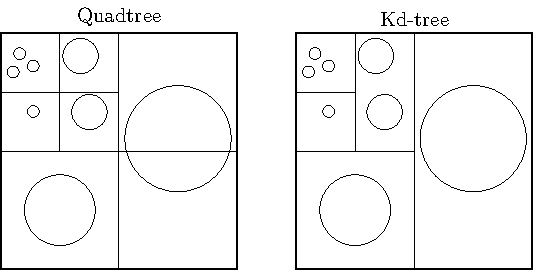
\includegraphics[width=\textwidth]{figures/SpaceVsData/SvsD}
% \end{frame}

\begin{frame}{Dangle and cut edges}
    \centering
    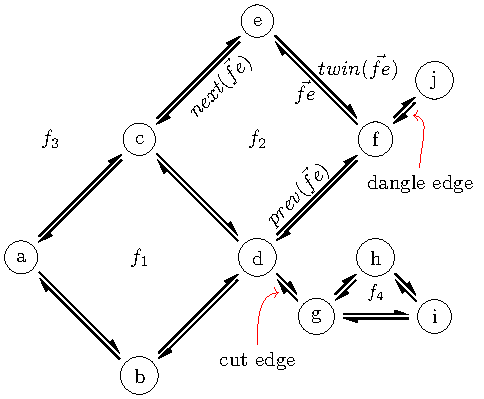
\includegraphics[width=0.6\textwidth]{../thesis/chapterExtension/dcel_example2}
\end{frame}

\begin{frame}{Dangle and cut edges}
    \centering

    \begin{tikzpicture}
    \node (A) {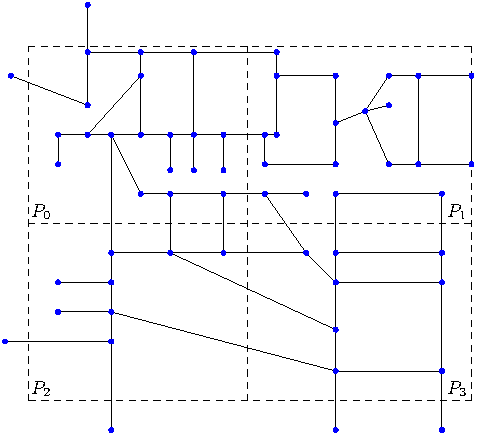
\includegraphics[width=0.8\textheight]{../thesis/chapterExtension/model/input/input}};
    \pause
    \draw[white, fill=white] (-4,-4) rectangle (4,4);
    \node (B) {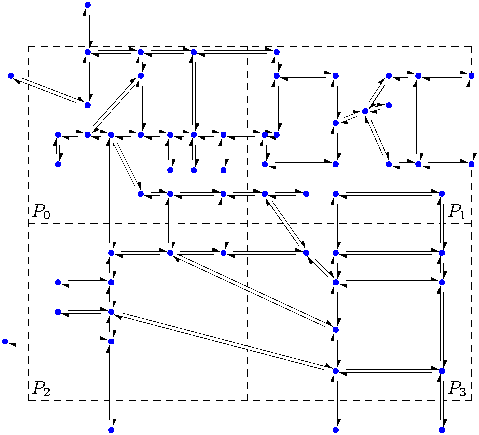
\includegraphics[width=0.8\textheight]{../thesis/chapterExtension/model/a/a}};
    \pause
    \draw[white, fill=white] (-4,-4) rectangle (4,4);
    \node (C) {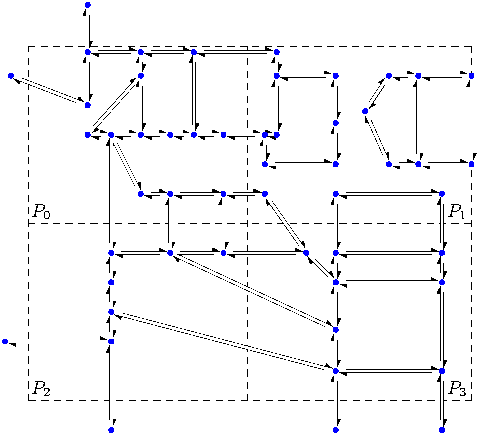
\includegraphics[width=0.8\textheight]{../thesis/chapterExtension/model/b/b}};
    \pause
    \draw[white, fill=white] (-4,-4) rectangle (4,4);
    \node (D) {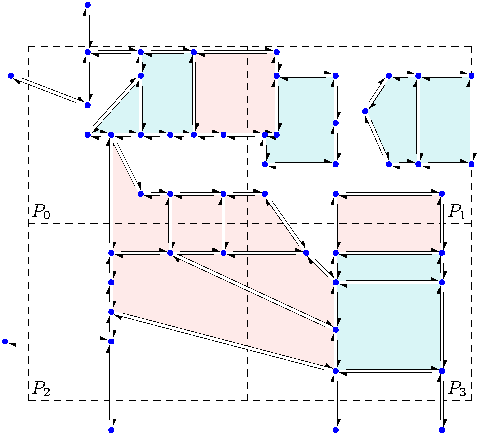
\includegraphics[width=0.8\textheight]{../thesis/chapterExtension/model/c/c}};
    \end{tikzpicture}
\end{frame}

\begin{frame}{Dangle and cut edges}
    \centering
    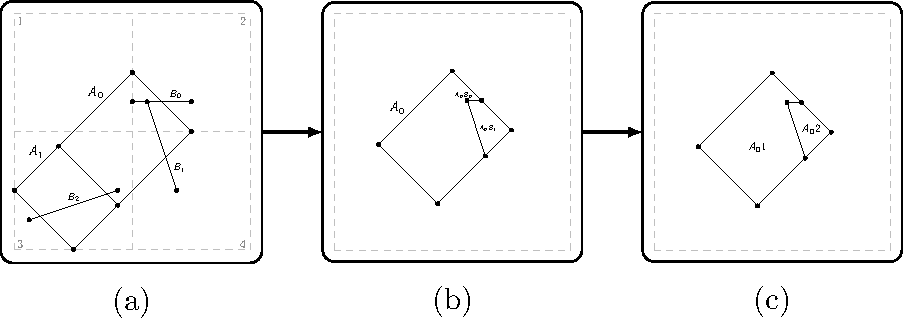
\includegraphics[width=\textwidth]{../thesis/chapterExtension/dangles_cuts/DAC}
\end{frame}

\begin{frame}{Dangle and cut edges}
    \centering
    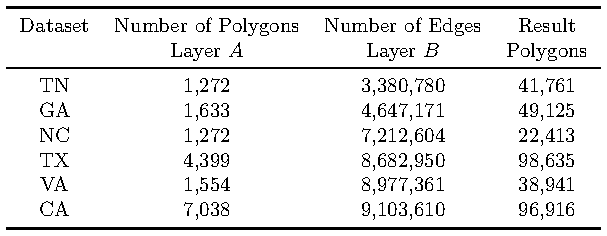
\includegraphics[width=0.85\textwidth]{figures/dangles_datasets}
\end{frame}

\begin{frame}{Dangle and cut edges}
    \centering
    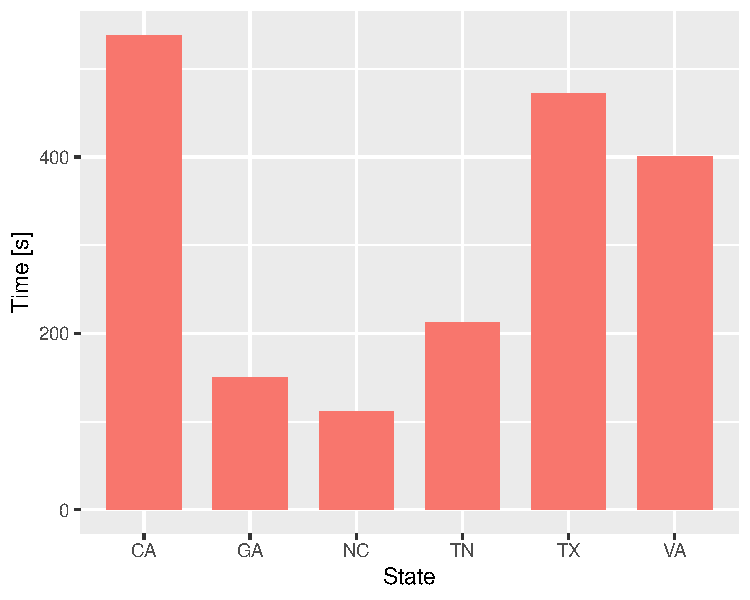
\includegraphics[width=0.75\textwidth]{../thesis/chapterExtension/states}
\end{frame}
